\documentclass[11pt]{article}
\usepackage{listings}
\lstset{language=Matlab,
breaklines=true,
keywordstyle=\color{blue},
identifierstyle=\color{black},
stringstyle=\color{mylilas},
commentstyle=\color{mygreen},
showstringspaces=false,
numbers=left,
numberstyle={\small \color{black}},
numbersep=9pt,
emph=[1]{for,end,break},
emphstyle=[1]\color{red}
}

\usepackage{color}
\definecolor{mygreen}{RGB}{28,172,0}
\definecolor{mylilas}{RGB}{170,55,241}

\usepackage{fancyhdr}
\pagestyle{fancy}
\newcommand\course{CSC 349A}
\newcommand\hwnumber{5}
\newcommand\duedate{November 19, 2019}

\lhead{Oliver Tonnesen\\V00885732}
\chead{\textbf{\Large Assignment \hwnumber}}
\rhead{\course\\\duedate}

\usepackage{graphicx}

\usepackage{algpseudocode}

\usepackage{mathtools}
\usepackage{amsmath}
\DeclareMathOperator{\fl}{fl}
\newenvironment{amatrix}[1]{%
  \left(\begin{array}{@{}*{#1}{c}|c@{}}
}{%
  \end{array}\right)
}


\begin{document}
\renewcommand{\thesubsection}{\thesection.\alph{subsection}}
\section{} % Section 1
\subsection{} % Section 1.a
\begin{align*}
	L_0(x)&=\frac{\left(x-\frac{\pi}{3}\right)\left(x-\frac{2\pi}{3}\right)\left(x-\pi\right)}
		{\left(0-\frac{\pi}{3}\right)\left(0-\frac{2\pi}{3}\right)\left(0-\pi\right)}\\
		&=\frac{-9x^3+18\pi x^2-11\pi^2x+2\pi^3}{2\pi^2}\\
	L_1(x)&=\frac{\left(x-0\right)\left(x-\frac{2\pi}{3}\right)\left(x-\pi\right)}
		{\left(\frac{\pi}{3}-0\right)\left(\frac{\pi}{3}-\frac{2\pi}{3}\right)\left(\frac{\pi}{3}-\pi\right)}\\
		&=\frac{27x^3-45\pi x^2+18\pi^2x}{2\pi^2}\\
	L_2(x)&=\frac{\left(x-0\right)\left(x-\frac{\pi}{3}\right)\left(x-\pi\right)}
		{\left(\frac{2\pi}{3}-0\right)\left(\frac{2\pi}{3}-\frac{\pi}{3}\right)\left(\frac{2\pi}{3}-\pi\right)}\\
		&=\frac{-27x^3+36\pi x^2-9\pi^2x}{2\pi^2}\\
	L_0(x)&=\frac{\left(x-0\right)\left(x-\frac{\pi}{3}\right)\left(x-\frac{2\pi}{3}\right)}
		{\left(\pi-0\right)\left(\pi-\frac{\pi}{3}\right)\left(\pi-\frac{2\pi}{3}\right)}\\
		&=\frac{9x^3-9\pi x^2+2\pi^2x}{2\pi^2}\\
\end{align*}

So we get

\begin{align*}
	P(x)&=\sum^3_{i=0} L_i(x)f(x_i)\\
	&=L_0(x)\cdot0+L_1(x)\cdot0.75+L_2(x)\cdot0.75+L_3(x)\cdot0\\
	&=0.75\left(L_1(x)+L_2(x)\right)\\
	&=\frac{0.75}{2\pi^3}\left(-9\pi x^2+9\pi^2x\right)\\
	&=\frac{-27\pi x^2+27\pi^2x}{8\pi^3}\\
	&=\frac{27x(\pi-x)}{8\pi^2}
\end{align*}


\subsection{} % Section 1.b
We execute the commands below
\lstinputlisting{mfiles/Q1b}
to get the following plot (the blue curve is $\sin^2x$, the red curve is the
polynomial interpolation):

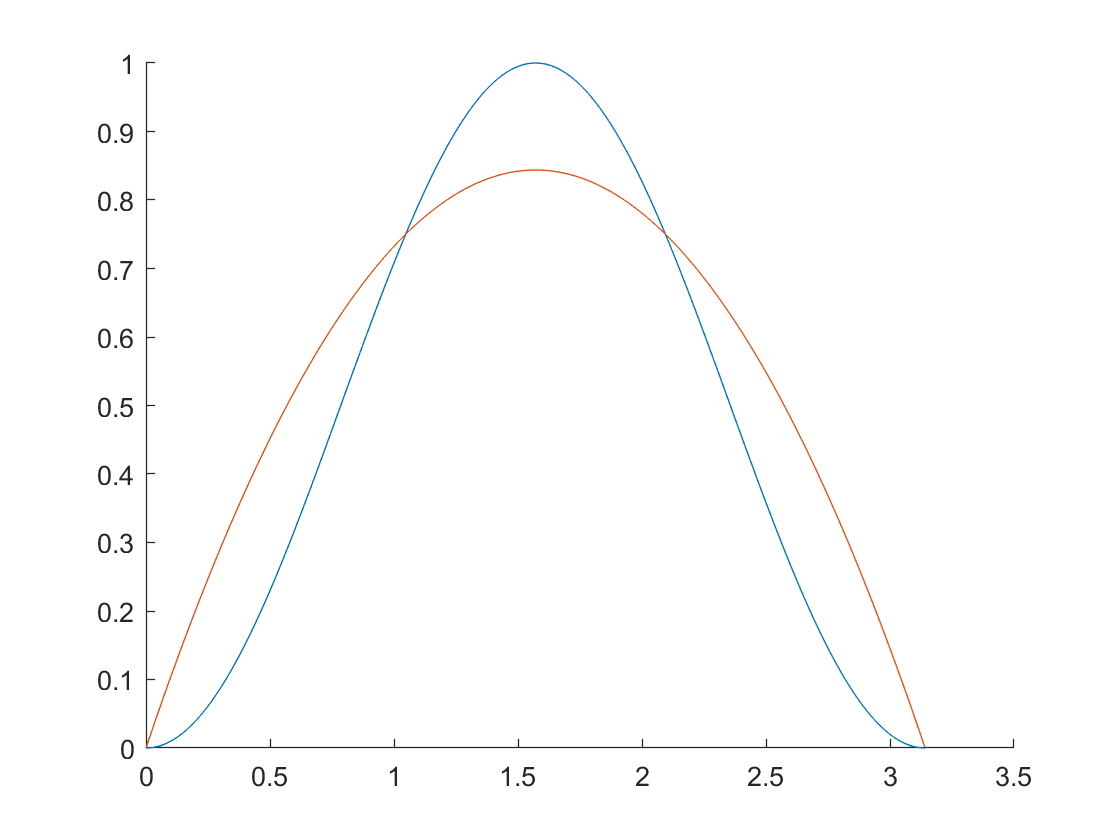
\includegraphics[scale=0.45]{q1b.png}


\section{} % Section 2
We have the following twelve conditions:

\begin{align*}
	\text{1: }&S_0(0)=\sin^2(0) & \text{2: }&S_1\left(\frac{\pi}{3}\right)=\sin^2\left(\frac{\pi}{3}\right)\\
	\text{3: }&S_2\left(\frac{2\pi}{3}\right)=\sin^2\left(\frac{2\pi}{3}\right) & \text{4: }&S_2(\pi)=\sin^2(\pi)\\
	\text{5: }&S_1\left(\frac{\pi}{3}\right)=S_0\left(\frac{\pi}{3}\right) & \text{6: }&S_2\left(\frac{2\pi}{3}\right)=S_1\left(\frac{2\pi}{3}\right)\\
	\text{7: }&S_1'\left(\frac{\pi}{3}\right)=S_0'\left(\frac{\pi}{3}\right) & \text{8: }&S_2'\left(\frac{2\pi}{3}\right)=S_1'\left(\frac{2\pi}{3}\right)\\
	\text{9: }&S_1''\left(\frac{\pi}{3}\right)=S_0''\left(\frac{\pi}{3}\right) & \text{10: }&S_2''\left(\frac{\pi}{3}\right)=S_1''\left(\frac{\pi}{3}\right)\\
	\text{11: }&S_0'(0)=2\sin0\cos0 & \text{12: }&S_2'(\pi)=2\sin\pi\cos\pi
\end{align*}

giving us twelve equations:

\begin{align*}
	\text{1: }&a_0=0 & \text{2: }&a_1=\frac{3}{4}\\
	\text{3: }&a_2=\frac{3}{4} & \text{4: }&a_2+b_2\left(\frac{\pi}{3}\right)+c_2\left(\frac{\pi}{3}\right)^2+d_2\left(\frac{\pi}{3}\right)^3\\
	\text{5: }&a_1-a_0-b_0\left(\frac{\pi}{3}\right)-c_0\left(\frac{\pi}{3}\right)^2-d_0\left(\frac{\pi}{3}\right)^3=0 &
		\text{6: }&a_2-a_1-b_1\left(\frac{\pi}{3}\right)-c_1\left(\frac{\pi}{3}\right)^2-d_1\left(\frac{\pi}{3}\right)^3=0\\
	\text{7: }&b_1-b_0-2c_0\left(\frac{\pi}{3}\right)-3d_0\left(\frac{\pi}{3}\right)^2=0 &
		\text{8: }&b_2-b_1-2c_1\left(\frac{\pi}{3}\right)-3d_1\left(\frac{\pi}{3}\right)^2=0\\
	\text{9: }&2c_1-2c_0-3d_0\left(\frac{\pi}{3}\right)=0 & \text{10: }&2c_2-2c_1-3d_1\left(\frac{\pi}{3}\right)=0\\
	\text{11: }&b_0=0 & \text{12: }&b_2+2c_2\left(\frac{\pi}{3}\right)+3d_2\left(\frac{\pi}{3}\right)^2=0\\
\end{align*}

We put these twelve equations together to get the below matrix, where the
columns, in order, represent $a_0,b_0,c_0,d_0,a_1,\ldots,d_2$:

$\begin{amatrix}{12}
	1 & 0 & 0 & 0 & 0 & 0 & 0 & 0 & 0 & 0 & 0 & 0 & 0\\
	0 & 0 & 0 & 0 & 1 & 0 & 0 & 0 & 0 & 0 & 0 & 0 & \frac{3}{4}\\
	0 & 0 & 0 & 0 & 0 & 0 & 0 & 0 & 1 & 0 & 0 & 0 & \frac{3}{4}\\
	0 & 0 & 0 & 0 & 0 & 0 & 0 & 0 & 1 & \frac{\pi}{3} & \left(\frac{\pi}{3}\right)^2 & \left(\frac{\pi}{3}\right)^3 & 0\\
	-1 & -\frac{\pi}{3} & -\left(\frac{\pi}{3}\right)^2 & -\left(\frac{\pi}{3}\right)^3 & 1 & 0 & 0 & 0 & 0 & 0 & 0 & 0 & 0\\
	0 & 0 & 0 & 0 & -1 & -\frac{\pi}{3} & -\left(\frac{\pi}{3}\right)^2 & -\left(\frac{\pi}{3}\right)^3 & 1 & 0 & 0 & 0 & 0\\
	0 & -1 & -2\frac{\pi}{3} & -3\left(\frac{\pi}{3}\right)^2 & 0 & 1 & 0 & 0 & 0 & 0 & 0 & 0 & 0\\
	0 & 0 & 0 & 0 & 0 & -1 & -2\frac{\pi}{3} & -3\left(\frac{\pi}{3}\right)^2 & 0 & 1 & 0 & 0 & 0\\
	0 & 0 & -2 & -3\frac{\pi}{3} & 0 & 0 & 2 & 0 & 0 & 0 & 0 & 0 & 0\\
	0 & 0 & 0 & 0 & 0 & 0 & -2 & -3\frac{\pi}{3} & 0 & 0 & 2 & 0 & 0\\
	0 & 1 & 0 & 0 & 0 & 0 & 0 & 0 & 0 & 0 & 0 & 0 & 0\\
	0 & 0 & 0 & 0 & 0 & 0 & 0 & 0 & 0 & 1 & 2\frac{\pi}{3} & 3\left(\frac{\pi}{3}\right) & 0\\
\end{amatrix}$


\section{} % Section 3
\subsection{} % Section 3.a
We use MATLAB to find the coefficients for the three cubic polynomials for our
spline interpolant:
\lstinputlisting{mfiles/Q3a}
and so our polynomials are:

\begin{align*}
	S_0(x)&\approx1.3678(x-0)^2-0.6531(x-0)^3\\
	S_1(x)&\approx0.75+0.7162\left(x-\frac{\pi}{3}\right)-0.6839\left(x-\frac{\pi}{3}\right)^2\\
	S_2(x)&\approx0.75-0.7162\left(x-\frac{2\pi}{3}\right)-0.6839\left(x-\frac{2\pi}{3}\right)^2+0.6531\left(x-\frac{2\pi}{3}\right)^3\\
\end{align*}


\subsection{} % Section 3.b
We use the following MATLAB statements 
\lstinputlisting{mfiles/Q3b}
to create the plot below, where the blue line is $\sin^2x$ and the red line is
the spline function:

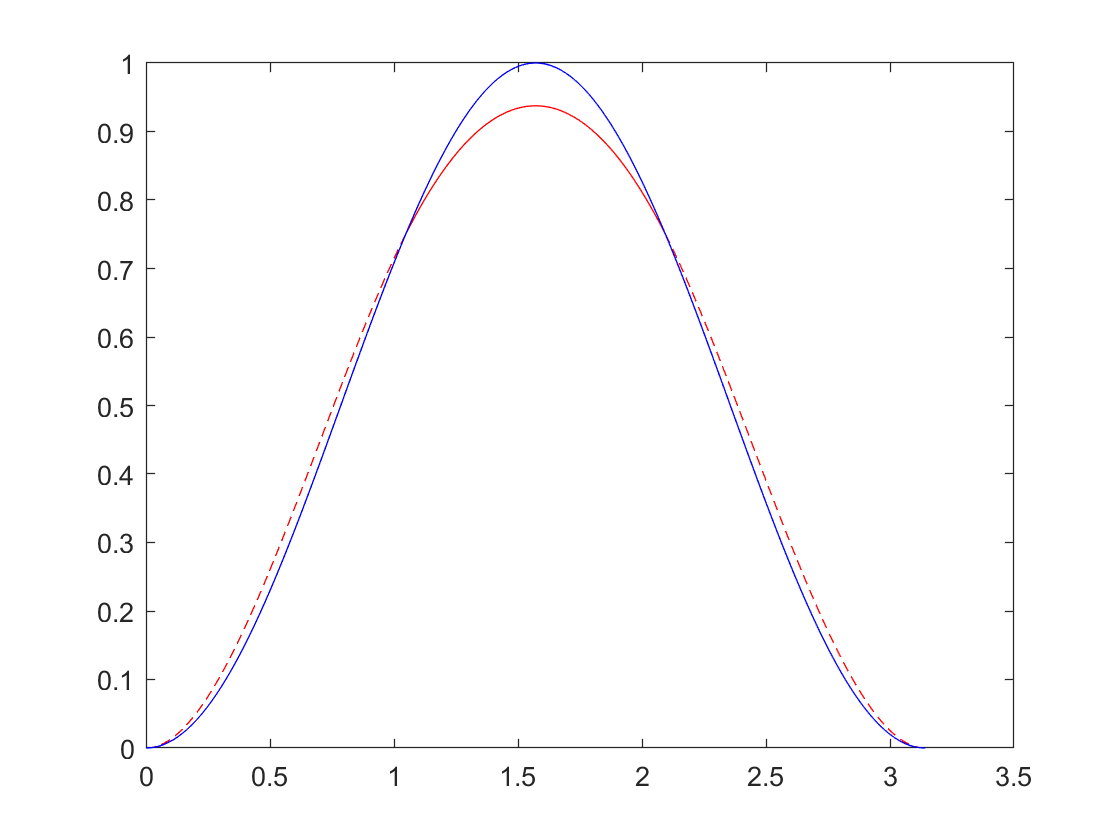
\includegraphics[scale=0.45]{q3b.png}



\end{document}
